\documentclass[runningheads]{llncs}
\usepackage[T1]{fontenc}
\usepackage{graphicx}
\usepackage{amsmath}
\usepackage{url}
\title{Multi-View Action Recognition Using TSN--GRU and Clip-Consistent Augmentation: A Course Project Report}
\titlerunning{Temporal Fusion and View Disentanglement}
\author{Vichanshu Raj \and Satwik Santosh \and Vishwas Pahwa \and Sudhanshu \and Kyan Mahajan \and Saumya Sood \and Akshat Parmar}
\authorrunning{IVP Group 19}
\institute{Image and Video Processing Course Project, Group 19}
\begin{document}
\maketitle
\begin{abstract}
Recognizing the same human action across camera viewpoints requires a representation that captures motion while limiting dependence on appearance and scene geometry. This paper consolidates two relevant approaches: the multi-branch temporal segment network integrated with a gated recurrent unit proposed by Bui and Nguyen, and DVANet proposed by Siddiqui, Tirupattur and Shah. The former aggregates ordered snippets and combines view-specific features; the latter separates action and view representations using transformer queries and supervised contrastive objectives. We compare their architectures, supervision, inference requirements, published evaluations and practical limitations. We further position a course-project implementation based on Inception-v3 and clip-consistent augmentation within this literature. The recorded project evaluation achieved 39.47\% on 418 target-view groups; a separately supplied local result is distinguished from that recorded run. Published scores are interpreted in the context of their protocols rather than combined into a single ranking. The analysis motivates controlled augmentation studies followed by representation-level view disentanglement.
\keywords{Multi-view action recognition \and Temporal segment networks \and GRU \and Disentanglement \and Contrastive learning}
\end{abstract}

\section{Introduction}
Human action recognition maps video observations to semantic action classes. A change in camera position can alter body configuration in the image, the visibility of an object and the background, even when the action remains unchanged. Multi-view learning can exploit complementary observations, but it also creates a risk: the representation may learn the camera or environment instead of the action. A robust system therefore needs both temporal modeling and an explicit account of viewpoint variation.

The two selected papers address different parts of this problem. Bui and Nguyen~\cite{bui} extend temporal segment networks (TSN) with view-specific branches and recurrent consensus. Siddiqui et al.~\cite{dva} introduce DVANet to disentangle action-relevant and view-relevant features. We ask three questions: how does each method represent temporal information, how is camera variation handled, and what can be concluded from the reported results? This is a comparative summary and course-project analysis, not a claim to reproduce DVANet.

\section{Literature Review of Both Papers}
\subsection{Multi-branch TSN with GRU}
TSN samples snippets from different temporal segments to cover an entire video without processing every frame~\cite{tsn}. Bui and Nguyen retain this sparse sampling principle and expand the network to multiple camera branches~\cite{bui}. A shared Inception-BN encoder extracts features common to the inputs. A separate $3\times3$ convolution block in each branch refines view-specific information. The authors replace average consensus with a shared GRU, retaining the last recurrent output as the video descriptor. Concatenation fuses the camera descriptors before classification.

The benefit of this design is its separation of shared appearance extraction, camera-specific refinement and order-sensitive temporal aggregation. Average consensus ignores the ordering of the sampled features; a GRU can use earlier snippets when processing later ones. However, concatenation alone does not force the fused descriptor to be invariant to camera position. The model also depends on the availability and pairing of camera clips during multi-branch training.

\subsection{DVANet}
DVANet uses a hybrid encoder--decoder architecture to learn separate action and view features~\cite{dva}. A video encoder produces spatiotemporal features, and a transformer decoder receives multiple learnable action queries and one view query. Action-query outputs are averaged into an action descriptor; the view query produces a separate view descriptor. Both descriptors receive classification supervision during training, whereas action prediction is used at inference.

The authors supplement classification with two contrastive losses and query orthogonality. The contrastive objectives encourage the same action from different cameras to be close in the action space, while videos from the same camera are close in the view space. This makes viewpoint an explicit factor of the learning objective rather than a nuisance that the classifier must implicitly ignore. The method requires view labels and carefully constructed training triplets. Its additional losses and queries also increase the implementation and tuning burden relative to a simple temporal fusion network.

\section{Methodology and Proposed Approach}
\subsection{Temporal and multi-view fusion}
Let a video from camera $v$ be divided into $K$ temporal segments. A snippet $T_{v,k}$ is sampled from segment $k$. With shared encoder $F$ and view-specific refinement $R_v$, the snippet representation is
\begin{equation}
z_{v,k}=R_v(F(T_{v,k})).
\end{equation}
The shared GRU aggregates snippets in chronological order:
\begin{equation}
h_{v,k}=\operatorname{GRU}(z_{v,k},h_{v,k-1}),\qquad
\hat y=\operatorname{softmax}(W[h_{1,K};\ldots;h_{V,K}]+b).
\end{equation}
These equations describe the reviewed design at a high level; they do not establish unpublished layer widths. In the paper's cross-view evaluation, two source cameras feed the two training branches. At testing, the unseen target-camera clip is duplicated into both branches~\cite{bui}. The duplication is an inference convention, not access to a second target-camera observation.

\subsection{Action--view disentanglement}
DVANet constructs a triplet consisting of an anchor $a$, a same-action video $s_a$ from another view, and a same-view video $s_v$ showing another action~\cite{dva}. The action-space objective decreases $D(f_a(a),f_a(s_a))$ relative to $D(f_a(a),f_a(s_v))$. The view-space objective reverses these roles: the same-view sample is positive and the same-action, different-view sample is negative. Thus, the two spaces are trained to retain different factors.

The total objective combines action and view cross-entropy, action and view contrastive terms, and an orthogonality term:
\begin{equation}
\mathcal L=\mathcal L_{a,ce}+\mathcal L_{v,ce}+\mathcal L_{a,c}
+\mathcal L_{v,c}+\mathcal L_{ortho}.
\end{equation}
The orthogonality term penalizes the absolute cosine similarity between distinct action queries. This discourages redundant queries but is not a guarantee of statistically independent representations. Triplet construction, loss balance and view supervision remain essential.

\subsection{Course-project approach}
The implemented extension is a practical augmentation study on the TSN--GRU architecture. It uses Inception-v3 instead of the paper's Inception-BN, four snippets per view, a $256$-dimensional refinement representation and a shared GRU with $128$ hidden units. These are project implementation choices, so the system should be described as an adaptation rather than an exact reproduction.

For each training clip, one horizontal-flip decision with probability $0.5$ is reused across its four frames. Independently, photometric augmentation is enabled with probability $0.5$: contrast is drawn from $[0.9,1.1]$ and brightness offset from $[-8,8]$ on the $0$--$255$ pixel scale. The settings are shared within a clip but drawn separately for each camera. Images are clipped to the valid range before ImageNet normalization. Validation and test use deterministic sampling without these transforms. Temporal consistency avoids artificial left--right changes between snippets, but flipping may still interact with camera geometry and should be tested in an ablation.

As a future extension, a view-classification or contrastive auxiliary objective could be added to the temporal model. This proposal is motivated by DVANet; it has not been implemented or evaluated in the submitted experiment.

\section{Comparative Analysis}
\begin{table}[t]
\caption{Conceptual comparison of the two selected papers.}
\centering\small
\begin{tabular}{p{2.4cm}p{4.1cm}p{4.1cm}}
\hline
Aspect & Multi-branch TSN--GRU & DVANet\\\hline
Temporal modeling & Sparse snippets; recurrent consensus & Spatiotemporal encoder and transformer decoder\\
View handling & Camera branches and late concatenation & Separate action/view queries and supervision\\
Training objective & Action classification & Classification, contrastive and orthogonality terms\\
Inference & Multi-branch fusion; duplicated target clip in cross-view setup & Action descriptor and action classifier\\
Main strength & Explicit snippet order; shared feature extraction & Direct pressure toward action--view separation\\
Main limitation & Fusion need not remove viewpoint information & Requires view labels, triplets and multiple objectives\\\hline
\end{tabular}
\end{table}

The methods should not be viewed simply as a small and a large version of the same network. Multi-branch TSN--GRU exploits complementary camera descriptors, while DVANet explicitly seeks to exclude view information from the action descriptor. Shared encoders reduce parameter duplication in the first method; contrastive supervision supplies additional learning signals in the second. Neither architecture by itself resolves dataset leakage, label errors or evaluation mismatch.

Computational cost cannot be ranked from architecture names alone. Sparse sampling limits the frames processed by TSN, but multiple camera branches increase per-action input. DVANet uses extra triplet videos during training but predicts actions from the action representation at inference. A fair efficiency comparison would report frames, resolution, hardware, batch size, parameter count and end-to-end latency under the same conditions. Such a matched benchmark is not available in this project.

\section{Results and Discussion}
\subsection{Published evidence}
Bui and Nguyen report 93.81\% action-level cross-subject accuracy on NUMA/N-UCLA with GRU consensus, compared with 88.49\% for their multi-branch model without GRU~\cite{bui}. Their three cross-view results are 82.58\%, 81.00\% and 89.76\%, with a reported mean of 84.4\%. They train for 80 epochs, starting at learning rate $0.001$ and reducing it at epochs 30 and 60. The authors explicitly caution that action-level and video-level comparisons are not directly equivalent.

DVANet reports 94.4\% cross-subject and 96.5\% cross-view accuracy on N-UCLA in Table 4~\cite{dva}. These numbers should not be subtracted directly from the three-split mean of the earlier paper to claim a controlled improvement: aggregation and protocol definitions must first be aligned. DVANet also evaluates NTU RGB+D, NTU RGB+D 120 and PKU-MMD. On PKU-MMD cross-subject, its full loss configuration reaches 95.8\%; removing both contrastive losses gives 94.2\%, and removing the orthogonality loss gives 95.0\%. These ablations support the usefulness of the training objectives in that setting rather than proving the same gain on every dataset.

\subsection{Project evidence and provenance}
The saved Kaggle outputs contain a completed 12-epoch development stage followed by a fresh 12-epoch refit. Subject 10 is held out from source-view pairs during development (43 validation samples). The refit uses all 418 complete source pairs and tests the unseen view-3 clip, duplicated into the two branches. The recorded final accuracy is $165/418=39.47\%$, macro-F1 is $0.3487$, and cross-entropy loss is $2.0077$. Predictions reproduce the stored accuracy and macro-F1. Development epoch 12 validation accuracy is 62.79\%; it is measured on a different set and must not be presented as target-view performance.

The historical presentation reports 36.6\% accuracy and 0.295 macro-F1 for the comparable target direction. The recorded difference is approximately 2.87 percentage points. This is descriptive evidence only: random training history, frame transformations and other implementation choices differ. A matched baseline across several seeds is necessary to attribute the change to augmentation.

The project owner separately supplies a local result of 78.47\% ($328/418$) and macro-F1 $0.7845$. These files are retained separately in the submission. Their execution provenance has not been independently established during packaging, and their stated historical reference of 69.6\% differs from the presentation's 36.6\%. Accordingly, this review does not use the local figure as verified evidence of a performance gain.

\begin{table}[t]
\caption{Results with explicit scope; rows are not a controlled ranking.}
\centering\small
\begin{tabular}{p{5.9cm}r p{2.7cm}}
\hline
Source and evaluation & Accuracy & Status\\\hline
TSN--GRU paper, three-split cross-view mean & 84.4\% & Published\\
DVANet paper, N-UCLA cross-view & 96.5\% & Published\\
Historical project, target view 3 & 36.6\% & Presentation/log\\
Augmented project, target view 3 & 39.47\% & Recorded Kaggle run\\
Separate local run, target view 3 & 78.47\% & Owner supplied\\\hline
\end{tabular}
\end{table}

Several limitations remain. The project uses fewer epochs and a different backbone from the base paper. Only one augmented target direction and one seed were evaluated in the recorded run. Grouping depends on matching action, subject and event identifiers across cameras; this correspondence requires independent dataset validation. Photometric jitter targets illumination variation but cannot synthesize unseen geometry or restore occluded evidence. These constraints motivate both careful experimental controls and representation-level extensions.


\section{Project Design and Data Workflow}
\subsection{System Requirements and Scope}
The implemented system accepts RGB video files and outputs an action prediction among ten classes. Its core components are video inventory, segment sampling, image preprocessing, model inference, and reporting of classification metrics. The prototype does not perform live person tracking, activity localization or surveillance event detection. The supplied demo accepts a single trimmed clip and applies the same input to both branches, consistent with the recorded target-view inference convention. A model score is displayed alongside the prediction; the score is a softmax output and is not a calibrated probability.

The data preparation and model scripts require a Python environment with PyTorch, torchvision, OpenCV, NumPy, pandas, scikit-learn, Matplotlib and seaborn. The recorded training run used a Tesla T4, CUDA and PyTorch 2.11. The demo loads a saved checkpoint and can run on CPU, although startup and inference are slower than on a GPU. No cloud connection is required for the demo once the dependencies, checkpoint and video are available. Training on Kaggle requires access to the dataset and ImageNet initialization weights.

\subsection{Dataset and Inventory}
The NW-UCLA dataset provides video from three Kinect viewpoints for ten subjects and ten action classes~\cite{data}. The local RGB archive used by the project contains 1,475 video files. The action identifiers present in the inventory are 1, 2, 3, 4, 5, 6, 8, 9, 11 and 12, which are mapped to contiguous classifier indices. Assuming that identifiers encode the same action instance across cameras, matching action, subject and event yields 418 groups with all three views. The original filename is retained in the manifest to make each split auditable. Event correspondence should be checked against the original source metadata before asserting temporal synchronization of every paired clip.

The paper by Bui and Nguyen reports 1,745 RGB videos, whereas the available archive has 1,475. Possible reasons for this discrepancy cannot be determined from the available files; counts should therefore be treated as properties of the respective reported data, not as proof that one copy is incomplete. The project's test set consists of the view-3 video in each of the 418 complete groups, not all view-3 videos in the archive. This restriction makes the group count comparable with the historical project run, but it excludes target clips that have no complete three-view group.

\subsection{Architecture and Execution Flow}
The implementation first decodes four frames from temporally ordered segments of each source video. OpenCV converts frames from BGR to RGB and resizes them to $224\times224$ pixels. Training samples a random frame inside each segment; validation and test choose the midpoint. Pixel values are scaled to $[0,1]$ and normalized using ImageNet mean and standard deviation. The implementation processes the resulting tensor as batch, view, time, channel, height and width.

The shared Inception-v3 trunk maps the flattened view and time dimensions to spatial feature maps. For each view, a separate convolution, batch normalization, rectified linear unit and global average pooling form the snippet feature. One GRU is shared between branches and receives snippet features in their original order. Final hidden states are concatenated, passed through dropout and mapped to ten action logits. The classification loss is cross entropy. In a cross-view test the target video is decoded once conceptually and supplied to both branches. The implementation performs this through two inputs from the same file; this does not introduce independent camera information.

\begin{figure}[t]
\centering
\fbox{\parbox{0.88\textwidth}{\centering
RGB videos from source views\\[2mm] $\downarrow$\\[2mm]
Inventory and group by action, subject and event\\[2mm] $\downarrow$\\[2mm]
Four ordered temporal segments per view\\[2mm] $\downarrow$\\[2mm]
Training-only clip-consistent augmentation\\[2mm] $\downarrow$\\[2mm]
Shared Inception-v3 $\rightarrow$ per-view refinement $\rightarrow$ shared GRU\\[2mm] $\downarrow$\\[2mm]
Concatenate branch features $\rightarrow$ ten action logits}}
\caption{Project data and model flow. During evaluation, training-only augmentation is bypassed; for cross-view testing the single target clip is supplied to both branches.}
\label{fig:flow}
\end{figure}

\subsection{Split and Augmentation Controls}
All 418 groups are first partitioned by subject for development: 375 source-view pairs train the model and 43 subject-10 pairs serve as validation. Each validation example retains both source views. Validation is evaluated at every epoch to expose training behavior; the target-view test is not used to select an epoch. After the fixed twelve-epoch development stage, a newly initialized model is trained on all 418 source pairs. Only this refit is used for the final cross-view evaluation.

The training augmentation combines clip-level horizontal flips and mild brightness/contrast changes. Applying the same geometric decision to all snippets of a clip avoids generating an artificial temporal switch in handedness or direction. It does not preserve a fixed physical relationship across the two source cameras because each clip draws its own decision. That trade-off should be evaluated separately before concluding that the transform improves multiview consistency. Brightness and contrast are similarly sampled once per clip. Validation and test have no random photometric or flip transformation. Augmentation does not add new action instances or unseen cameras to the dataset.

\subsection{Metrics and Reproducibility}
Accuracy is the number of correct predictions divided by the number of evaluated examples. For each class, precision is true positives divided by predicted positives and recall is true positives divided by true examples. Class F1 is the harmonic mean of precision and recall; macro-F1 is the unweighted mean over all ten classes. Undefined values are assigned zero by the evaluation code. The confusion matrix records the true class in rows and predicted class in columns. This convention allows a reader to distinguish frequent misclassifications from classes with low support.

The run fixes the random seed to 42, uses batch size 2 and optimizes the model with stochastic gradient descent, momentum 0.9 and weight decay $5\times 10^{-4}$. The twelve-epoch schedule starts at $10^{-3}$ and reduces learning rate by ten after epochs 4 and 9. These are project settings, not the paper's 80-epoch schedule. A fixed seed makes the configuration easier to repeat, but one run does not characterize variation from initialization, data order, GPU kernels or held-out subjects.

\subsection{Integrity Checks and Error Handling}
The archive, expected folder hierarchy and inventory should be checked before training. The code rejects duplicate view entries and stops if a video cannot be opened or a selected frame cannot be decoded. This is preferable to silently inserting an all-black frame because a decode failure could otherwise become a feature or distort the measured accuracy. The split manifest preserves action, subject, event and video paths for investigation. The packaged audit recomputes accuracy from the predictions and verifies the expected count.

The demonstration loads a checkpoint using its architecture and class mapping, decodes the selected video, samples four frames and displays the top predicted class. A failed video read produces an error message. The test is a functional demonstration of the pipeline, not proof of accuracy on arbitrary internet video. Camera viewpoint, temporal duration, motion and background outside the dataset may differ substantially from the training conditions.

\section{Detailed Experimental Analysis}
\subsection{Development Learning Curves}
The development model starts at 18.93\% training accuracy and 30.23\% validation accuracy in epoch 1. By epoch 12, training accuracy is 82.93\%, training loss is 0.6906, validation accuracy is 62.79\%, and validation macro-F1 is 0.5674. The validation accuracy is not monotonic: it is 67.44\% at epoch 2 and 41.86\% at epoch 4, then rises again. With only 43 validation groups, one additional correct prediction changes accuracy by approximately 2.33 percentage points. The small support limits the precision with which model selection or generalization can be inferred.

The source-subject split tests generalization to a held-out actor using source cameras. The final cross-view split tests a different question: target-camera performance, with subject identities also present among training source views. Thus, the two values cannot be treated as measurements of the same held-out condition. Reporting the development score as the final unseen-camera result would conflate the protocols.

\begin{figure}[t]
\centering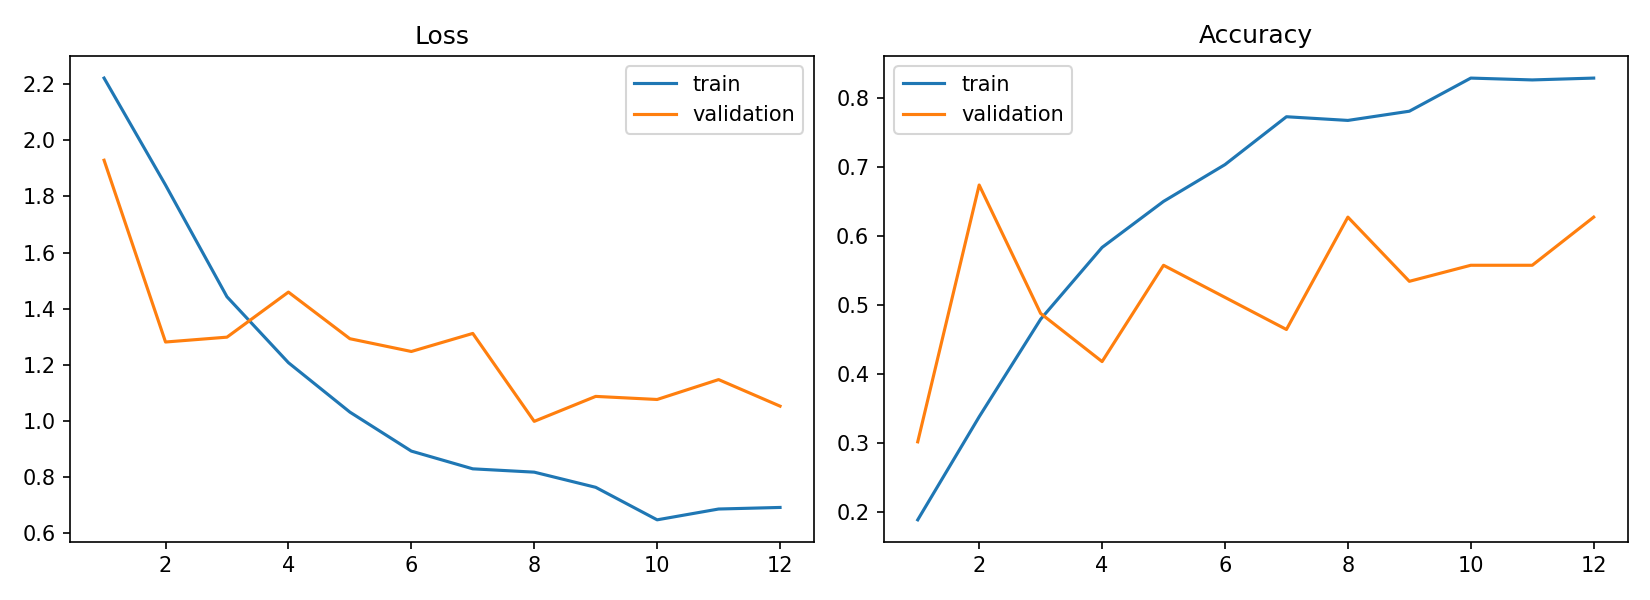
\includegraphics[width=0.95\textwidth]{learning_curves.png}
\caption{Recorded development training and subject-10 validation curves. The validation set contains 43 source-view pairs.}
\label{fig:curves}
\end{figure}

\subsection{Refit and Final Cross-View Evaluation}
After development, the model is reinitialized and trained on all 418 source pairs. Its training accuracy reaches 82.54\% at epoch 12. Inference on the held-out view-3 clips yields 165 correct predictions out of 418, for 39.47\% accuracy. Macro precision and macro recall computed from the prediction file are 0.3717 and 0.3914 respectively; macro-F1 stored by the run is 0.3487. The discrepancy between training accuracy and target-view accuracy is consistent with difficulty transferring to the unseen camera, although a training/test gap alone cannot establish the cause.

The confusion matrix in Fig.~\ref{fig:cm} is generated by the recorded evaluation. Off-diagonal counts show how errors distribute among the ten action classes. Class-level analysis is useful for determining whether the system struggles with semantically related movements, but the small size and subject overlap should be considered before drawing operational conclusions. No claim is made that the classifier is suitable for safety-critical decisions or that the listed probabilities are calibrated.

\begin{figure}[t]
\centering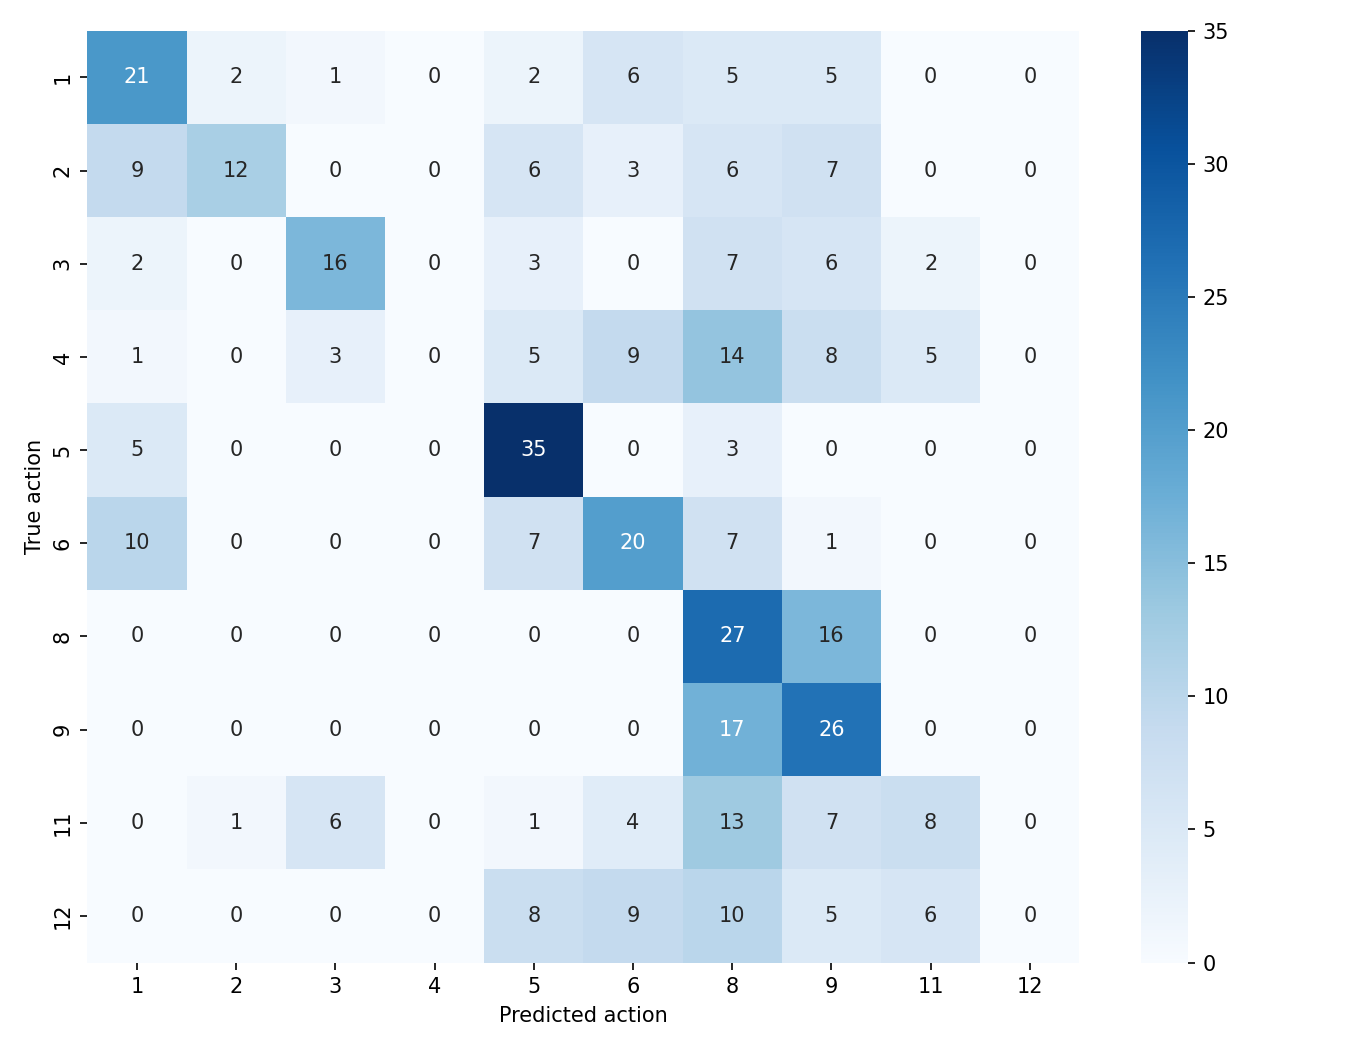
\includegraphics[width=0.85\textwidth]{confusion_matrix.png}
\caption{Recorded target-view confusion matrix; rows denote true classes and columns predictions. Action identifiers follow the dataset filenames.}
\label{fig:cm}
\end{figure}

\subsection{Historical Comparison and Interpretation}
The historical implementation reported in the earlier presentation obtains 36.6\% for the same source and target camera direction on 418 groups. The recorded augmented experiment gives 39.47\%, a difference of approximately 2.87 percentage points. This should not be interpreted as a reliable estimated augmentation effect: the original run used frame-level flips, different random number histories and a different overall experiment sequence. An ablation would train a baseline and each augmentation variant under an otherwise fixed configuration, repeat each seed, and reserve the target test set for the fixed final comparison.

The current project does not reproduce the base paper's 89.76\% for {1,2} to 3. The paper used Inception-BN and 80 training epochs, whereas the reported adaptation uses Inception-v3 and twelve epochs. The split membership, image preprocessing and training details may differ as well. The gap is informative for project development but cannot be assigned to any one design choice without controlled experiments.

\subsection{Ablation and Validation Plan}
A useful sequence is to begin with the same sampling, preprocessing, backbone and split without new photometric augmentation. A second condition changes only the horizontal flip from independently sampled frames to a shared clip-level decision. A third adds brightness and contrast. Repeating these conditions with at least three seeds would show whether any change is stable. Subject-level validation can guide choices; the target-view split should be evaluated only after the configuration is fixed. Scores should be accompanied by support counts and class-level precision, recall and confusion matrices.

Additional testing should examine the correspondence of paired filenames, decode failures, low-frame-count clips, normalization and model loading. Training should save the exact data manifests, hyperparameters and model checkpoint. Latency should distinguish model-only time from decoding and preprocessing. These steps make an experiment reproducible and expose sources of variation that a single final accuracy cannot capture.

\subsection{Proposed Extension from DVANet}
One possible extension would attach an auxiliary view classifier to a feature that is separated from the action descriptor. The same-action/different-view and same-view/different-action examples used by DVANet motivate a contrastive training scheme, but their construction requires reliable camera labels. This extension should be compared with the augmentation-only model under the same splits and evaluation process. It has not been implemented in the present project, and no performance gain is claimed for it.


\section{Conclusion and Future Scope}
Temporal fusion and view disentanglement provide complementary responses to multi-view action recognition. TSN--GRU emphasizes coverage of the video and order-aware aggregation; DVANet uses explicit action/view representations and structured supervision to reduce viewpoint interference. Their reported results support these ideas within their respective protocols, while the project demonstrates the practical difficulty of reproducing them under reduced training budgets.

The next steps are a matched augmentation ablation over multiple seeds, complete cross-view evaluation, verification of camera pairing, and reporting of precision, recall, macro-F1 and latency with confidence intervals. A subsequent research extension may combine recurrent temporal descriptors with action/view supervision. Claims about that extension must follow implementation and evaluation rather than precede them.

\begin{thebibliography}{4}
\bibitem{bui} A.-V. Bui and T.-O. Nguyen, ``Multi-view human action recognition based on TSN architecture integrated with GRU,'' \textit{Procedia Computer Science}, vol. 176, pp. 948--955, 2020. \url{https://doi.org/10.1016/j.procs.2020.09.090}
\bibitem{dva} N. Siddiqui, P. Tirupattur, and M. Shah, ``DVANet: Disentangling view and action features for multi-view action recognition,'' in \textit{Proceedings of the AAAI Conference on Artificial Intelligence}, vol. 38, pp. 4873--4881, 2024.
\bibitem{tsn} L. Wang et al., ``Temporal segment networks: Towards good practices for deep action recognition,'' in \textit{Computer Vision -- ECCV 2016}, Springer, 2016, pp. 20--36.
\bibitem{data} J. Wang et al., ``Cross-view action modeling, learning, and recognition,'' in \textit{Proceedings of the IEEE Conference on Computer Vision and Pattern Recognition}, 2014, pp. 2649--2656.
\end{thebibliography}
\end{document}
